\documentclass[show notes]{beamer}
\usetheme{Rochester}

\usepackage[utf8]{inputenc}
\usepackage[english]{babel}

\usepackage{graphicx}
\usepackage{amsmath,amssymb}
\usepackage{ gensymb }

\title{Advanced Projects in Exoplanets}
\subtitle{The RM Effect}
\author{Dina Sofia Mortensen \& Jesper Dam Knudgaard}
\institute{Stellar Astrophysics Centre, Aarhus University}
\date{\today}

\begin{document}

\begin{frame}
\titlepage
\end{frame}

\section{The RM Effect}

\begin{frame}
\frametitle{Transiting Exoplanets}
	\begin{figure}
		\centering
		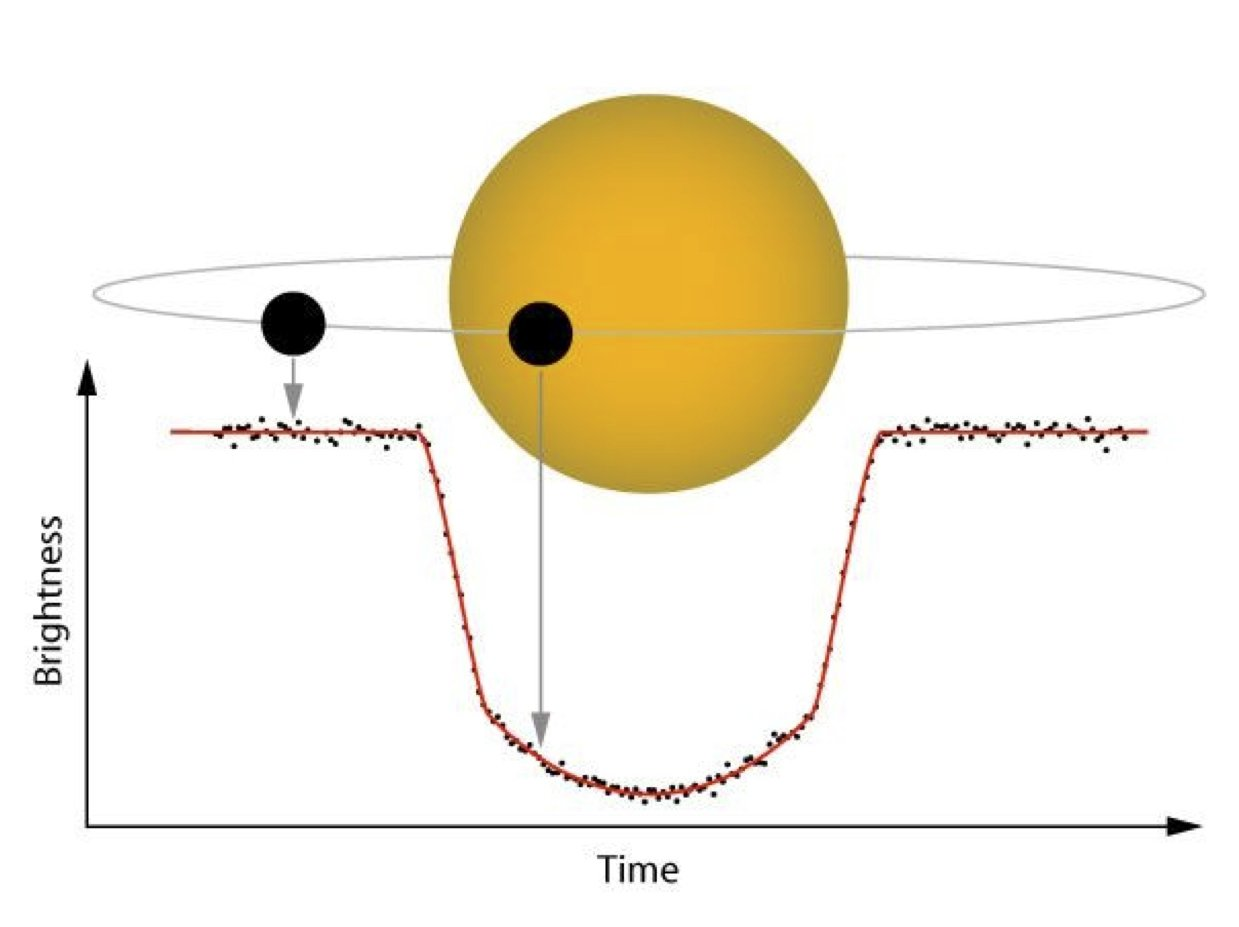
\includegraphics[width = 0.7\columnwidth]{../figures/Transit.jpg}
		\caption{\textit{Credit ESO}}
		\label{fig:transit} 
	\end{figure}
\end{frame}

\begin{frame}
\frametitle{Rossiter-McLaughlin Effect}
	\begin{figure}
		\centering
		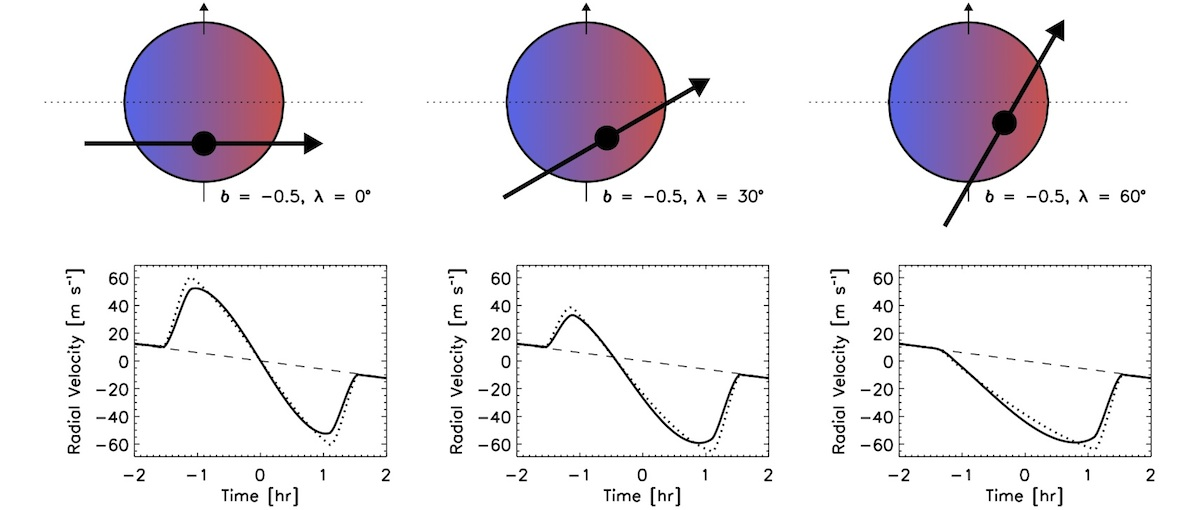
\includegraphics[width=\textwidth]{../figures/winnwhites.jpg}
		\caption{\url{https://wasp-planets.net/tag/rossiter-mclaughlin-effect/}}
		\label{fig:rm_effect}
	\end{figure}
\end{frame}

\note{Husk at nævne at det kun er projiceret obliquity vi kan måle, og det er fordi vi ikke ved hvordan stjernens rotationsakse er inklineret i forhold til os. }

\begin{frame}
\frametitle{}

\end{frame}

\section{Our Model}

\begin{frame}
\frametitle{Our Model - Linear}
\begin{columns}
	\column{0.5\textwidth}
		Planet moves in straight line in front of the star\\
		
		This path is determined by:
		\begin{itemize}
			\item Projected obliquity
			\item Impact parameter
		\end{itemize}
		
		This model is not physical
		
	\column{0.5\textwidth}

\end{columns}
\end{frame}


\begin{frame}
\frametitle{Keplers Equations}	

To get $r(t)$:

Calculate mean anomaly:
\begin{equation*}
M(t) = \sqrt{\frac{G (M_\star + M_p)}{a^3}} \cdot (t - t_p).
\end{equation*}

Calculate eccentric anomaly by numerical iteration:
\begin{equation*}
E_{n+1} = E_n - \frac{E_n - e sin(E_n) - M(t)}{1 - e sin(E-n)}.
\end{equation*}

Calculate true anomaly:
\begin{equation*}
\nu(t) = 2 \tan^{-1}( \left(\frac{1+e}{1-e}\right)^{1/2} \tan(E(t)/2) ).
\end{equation*}

Calculate separation:
\begin{equation*}
r(t) = a \frac{1 - e^2}{1 + e cos(\nu(t)}.
\end{equation*}

\end{frame}


\begin{frame}
\frametitle{Our Model - Physical version}
\begin{columns}
	\column{0.5\textwidth}
		Planet orbits the star.\\
		
		Keplers equation is solved for input parameters.\\

		The path is determined by:\\
		 $ a $, $ e $, $ i $, $ \omega $, $ M_{\star} $, $ M_p $, $ t_p $, $ \lambda $, $ R_p/R_{\star} $ and $ v\sin(i_{\star}) $.\\
		
		Much more resource heavy, but also correct
		
	\column{0.5\textwidth}
		\begin{figure}
			\centering
			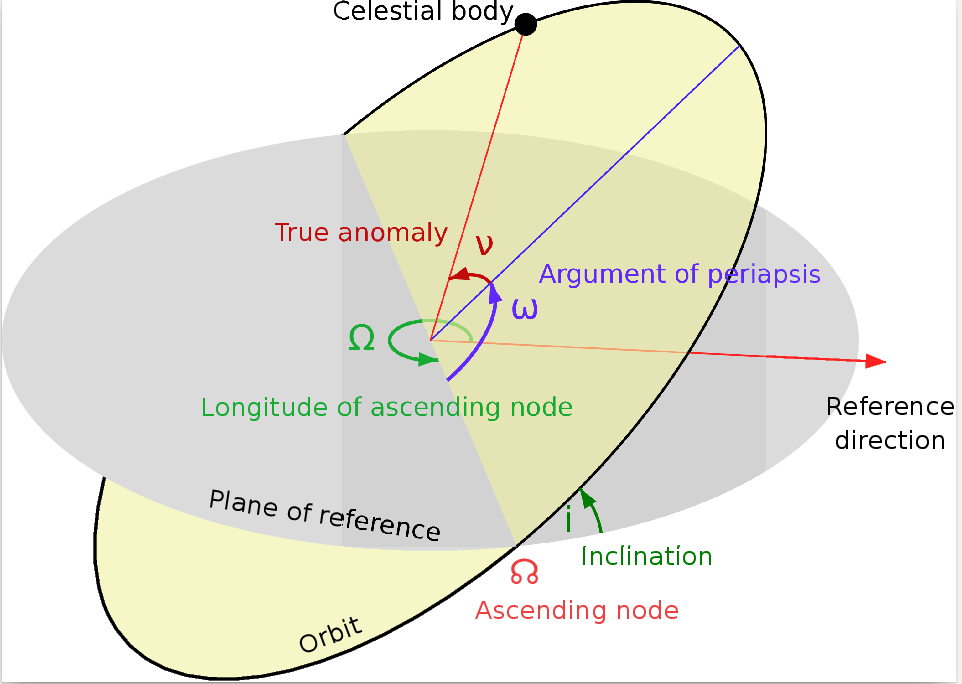
\includegraphics[width=\textwidth]{../figures/kepler.png}
			\caption{Credit: Wikipedia user Lassuncty}
			\label{fig:orbit}
		\end{figure}
\end{columns}

\end{frame}

\begin{frame}
\frametitle{Modelling Planet Orbit}
Calculate projected coordinates of the planet:

\begin{align*}
X_i& = -r cos(\omega + \nu), \\
Y_i& = -r sin(\omega + \nu) cos(i).
\end{align*}

\begin{align*}
X& = X_i cos(\lambda) + Y_i sin(\lambda), \\
Y& = -X_i sin(\lambda) + Y_i cos(\lambda), \\
Z& = r sin(\omega + \nu) sin(i).
\end{align*}
\end{frame}

\note{Vi laver her antagelsen at transit midpunkt sker til tiden t=0, og at $ \omega=90 $, så i tilfældet hvor vi har en eccentricitet, vil transitten ske ved periapsis.}

\begin{frame}
\frametitle{Our Model - Outputs}
	[Video here]
\end{frame}

\begin{frame}
\frametitle{Our Model - Outputs}

\begin{figure}
\centering
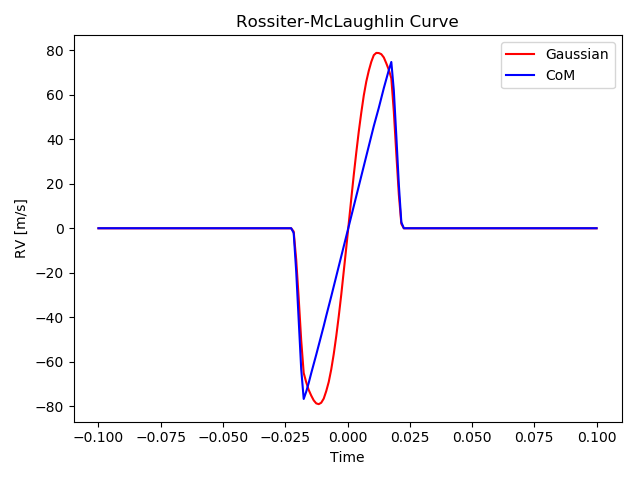
\includegraphics[width=0.9\textwidth]{../figures/animation1_rmcurve.png}
\end{figure}

\end{frame}

\begin{frame}
\frametitle{Our Model - Outputs}

\begin{figure}
\centering
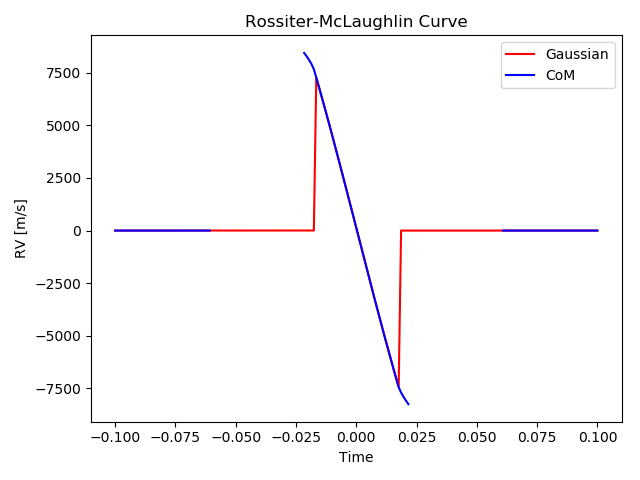
\includegraphics[width=0.9\textwidth]{../figures/animation2_rmcurve.png}
\end{figure}

\end{frame}

\begin{frame}
\frametitle{Data}
\begin{columns}
	\column{0.5\textwidth}
	
	
	\column{0.5\textwidth}
	\begin{figure}
		\centering
		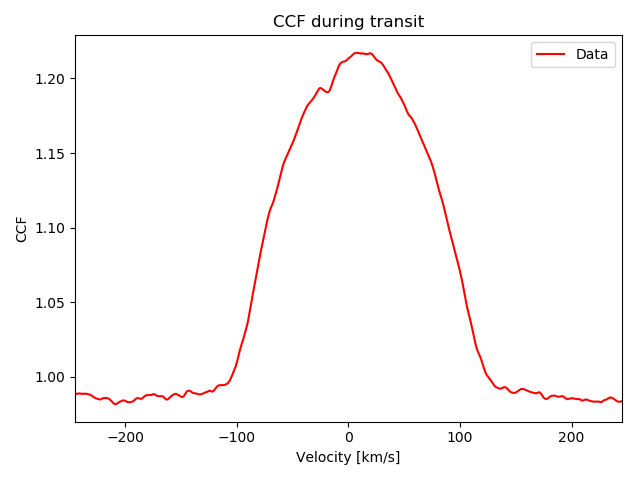
\includegraphics[width=\textwidth]{../figures/CCF_it.png}
		\label{fig:CCF_it}
	\end{figure}	
\end{columns}
\end{frame}

\begin{frame}
\frametitle{Data - The stellar line}
\begin{figure}
	\centering
	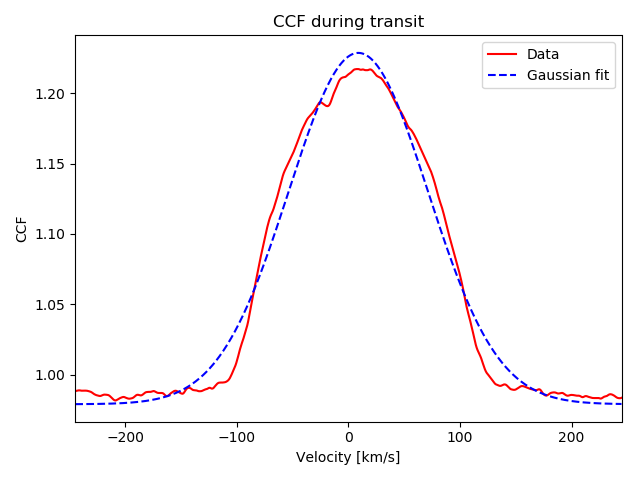
\includegraphics[width=0.8\textwidth]{../figures/CCF_it_fit.png}
	\label{fig:CCF_fit}
\end{figure}
\end{frame}

\begin{frame}
\frametitle{Data - The Transit}
\begin{figure}
	\centering
	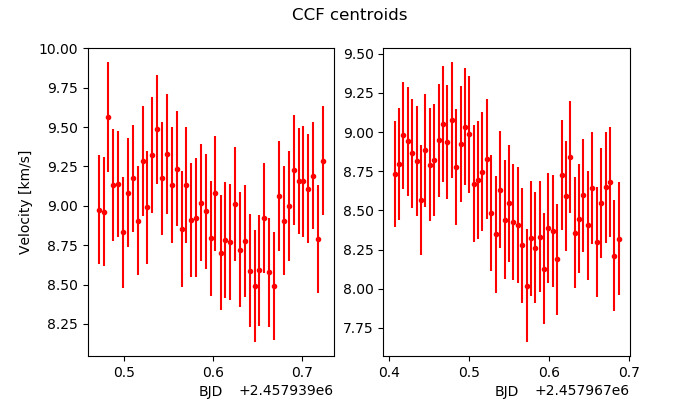
\includegraphics[width=\textwidth]{../figures/ccf_centroids.png}
	\label{fig:CCF_cent}
\end{figure}
\end{frame}

\begin{frame}
\frametitle{Data - The 'Planet Line'}
\begin{figure}
	\centering
	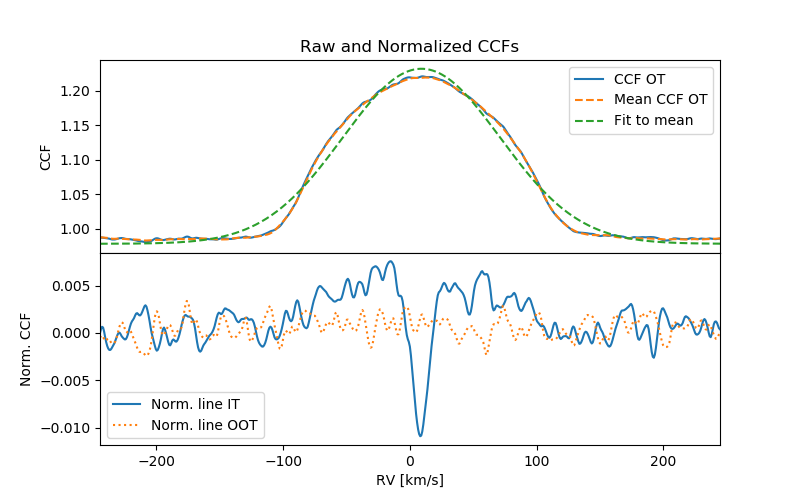
\includegraphics[width=\textwidth]{../figures/ccfs_norm.png}
	\label{fig:CCFs_norm}
\end{figure}
\end{frame}

\begin{frame}
\frametitle{Data - The RM-effect}
	\begin{figure}
	\centering
	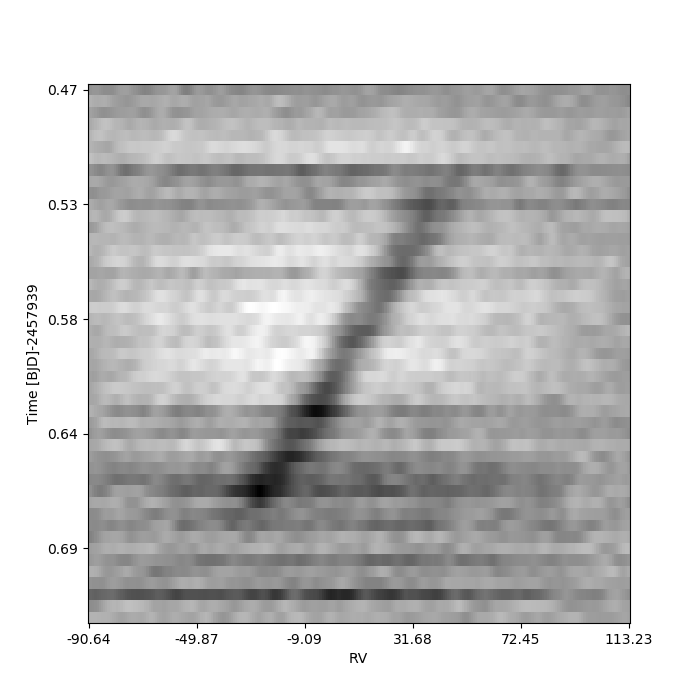
\includegraphics[width=\textwidth]{../figures/Colormap.png}
	\label{fig:colormap}
\end{figure}
\end{frame}


\begin{frame}
\frametitle{Data}
	\begin{figure}
	\centering
	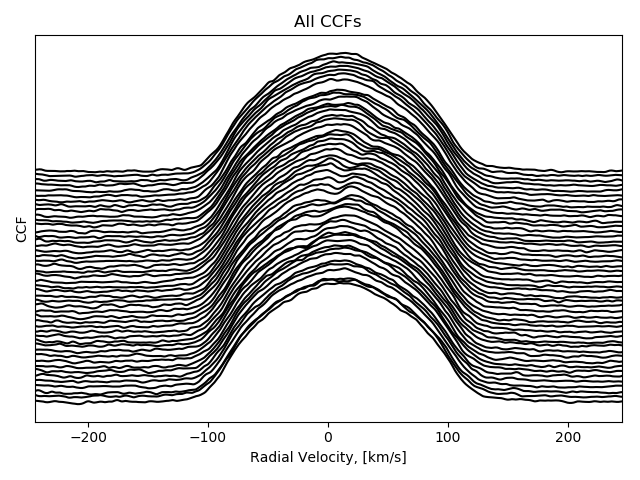
\includegraphics[width=0.8\textwidth]{../figures/All_CCFs.png}
	\label{fig:all_ccfs}
\end{figure}
\end{frame}


\begin{frame}
\frametitle{Data - Fit to CCF}
\begin{figure}
	\centering
	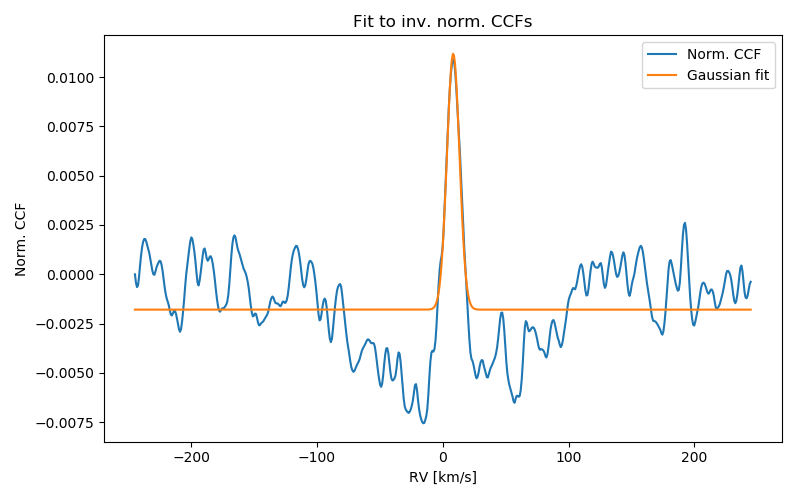
\includegraphics[width=\textwidth]{../figures/fitted_ccf.png}
	\label{fig:fitted_ccf}
\end{figure}
\end{frame}

\begin{frame}
\frametitle{Data - RM curve}
	\begin{figure}
		\centering
		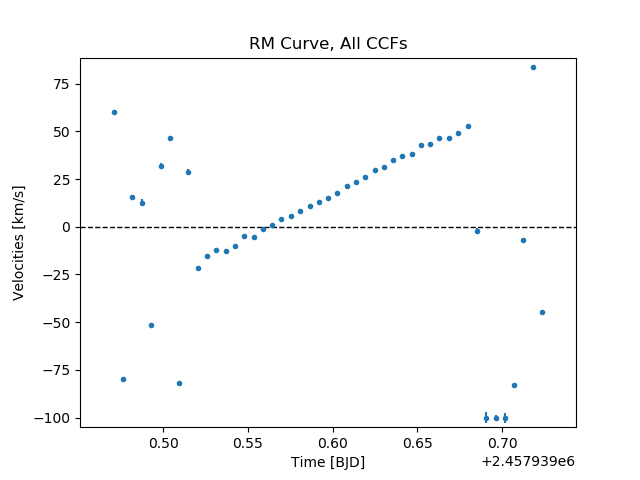
\includegraphics[width=0.8\textwidth]{../figures/RM_all_CCFs.png}
		\label{fig:RM_all_CCFs}
	\end{figure}
\end{frame}


\begin{frame}
\frametitle{Data - RM curve}
\begin{figure}
	\centering
	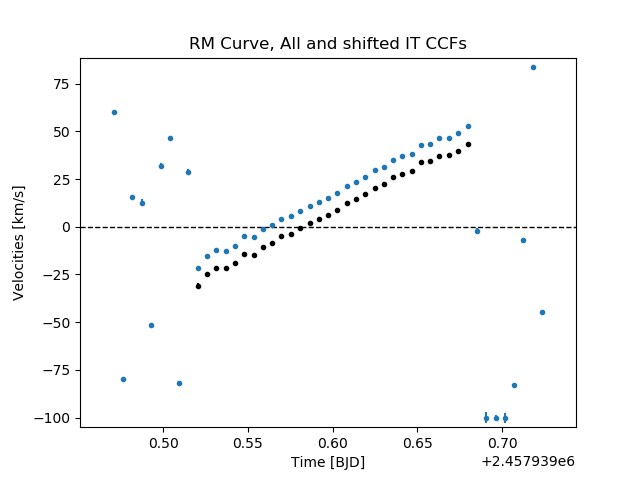
\includegraphics[width=0.8\textwidth]{../figures/RM_all_shift.png}
	\label{fig:RM_all_shift}
\end{figure}
\end{frame}

\begin{frame}
\frametitle{Data - RM curve}
\begin{figure}
	\centering
	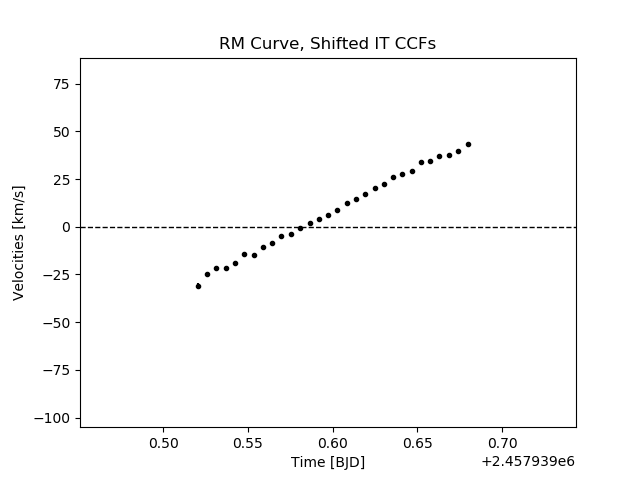
\includegraphics[width=0.8\textwidth]{../figures/RM_shift.png}
	\label{fig:RM_shift}
\end{figure}
\end{frame}

\section*{The Fit}

\begin{frame}
\frametitle{The Fit - System Parameters}
\begin{columns}
	\column{0.5\textwidth}
	Variables:
	\begin{itemize}
	\item $\lambda$
	\item $\omega$
	\item $v \sin(i_\star)$
	\end{itemize}
	\column{0.5\textwidth}
	Constants:
	\begin{itemize}
	\item $t_p = 0$
	\item $a = 4.756 R_\star$
	\item $e = 0$
	\item $M_\star = 1.72 M_\odot$
	\item $M_p = 3.7 M_J$
	\item $\frac{R_p}{R_\star} = 0.0735$
	\item $\omega = 90 \degree$
	\end{itemize}
\end{columns}
\end{frame}

\begin{frame}
\frametitle{Fitting with curvefit}
\begin{figure}
\centering
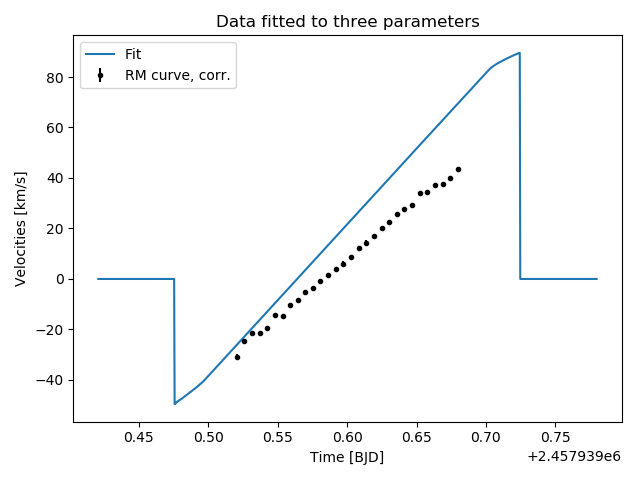
\includegraphics[width=0.9\textwidth]{../figures/curve_fit_rmcurve.png}
\end{figure}
\end{frame}

\begin{frame}
\frametitle{Linear fit}
\end{frame}


\end{document}
